%; whizzy chapter
% -initex iniptex -latex platex -format platex -bibtex jbibtex -fmt fmt
% $B0J>e(B whizzytex $B$r;HMQ$9$k>l9g$N@_Dj(B.

%     Kansai Debian Meeting resources
%     Copyright (C) 2007 Takaya Yamashita
%     Thank you for Tokyo Debian Meeting resources

%     This program is free software; you can redistribute it and/or modify
%     it under the terms of the GNU General Public License as published by
%     the Free Software Foundation; either version 2 of the License, or
%     (at your option) any later version.

%     This program is distributed in the hope that it will be useful,
%     but WITHOUT ANY WARRANTY; without even the implied warranty of
%     MERCHANTABILITY or FITNESS FOR A PARTICULAR PURPOSE.  See the
%     GNU General Public License for more details.

%     You should have received a copy of the GNU General Public License
%     along with this program; if not, write to the Free Software
%     Foundation, Inc., 51 Franklin St, Fifth Floor, Boston, MA  02110-1301 USA

%  preview (shell-command (concat "evince " (replace-regexp-in-string "tex$" "pdf"(buffer-file-name)) "&"))
% $B2hA|%U%!%$%k$r=hM}$9$k$?$a$K$O(B ebb $B$rMxMQ$7$F(B boundingbox $B$r:n@.(B.
%(shell-command "cd image200708; ebb *.png")

%%$B$3$3$+$i%X%C%@3+;O(B.

\documentclass[mingoth,a4paper]{jsarticle}
\usepackage{kansaimonthlyreport}
\usepackage[dvips]{xy}
\usepackage{ascmac}

% $BF|IU$rDj5A$9$k(B, $BKh7nJQ$o$j$^$9(B.
\newcommand{\debmtgyear}{2011}
\newcommand{\debmtgmonth}{09}
\newcommand{\debmtgdate}{25}
\newcommand{\debmtgnumber}{51}

\begin{document}

\begin{titlepage}

% $BKh7nJQ99$9$kItJ,(B, $BK\J8$NKvHx$b=$@5$9$k$3$H$r$o$9$l$:$K(B

 $BBh(B\debmtgnumber{}$B2s(B $B4X@>(B Debian $BJY6/2q;qNA(B

\vspace{2cm}

\begin{center}
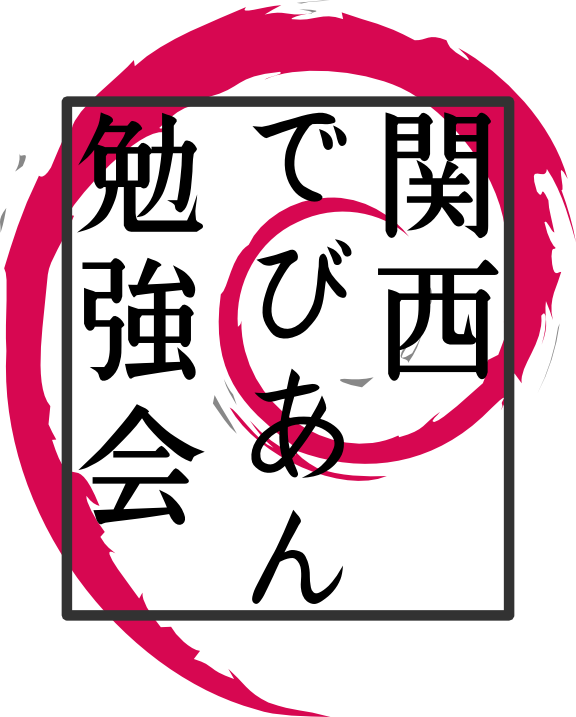
\includegraphics{image200802/kansaidebianlogo.png}
\end{center}

\begin{flushright}
\hfill{}$B4X@>(B Debian $BJY6/2qC4Ev<T(B $B:4!9LZ!&ARI_!&$N$,$?(B \\
\hfill{}\debmtgyear{}$BG/(B\debmtgmonth{}$B7n(B\debmtgdate{}$BF|(B
\end{flushright}

\thispagestyle{empty}
\end{titlepage}

\dancersection{Introduction}{Debian JP}

\subsection*{}%$B%m%4MQ$N%9%Z!<%92T$.(B

$B4X@>(B Debian $BJY6/2q$O(B Debian GNU/Linux $B$N$5$^$6$^$J%H%T%C%/(B ($B?7$7$$%Q%C%1!<(B
$B%8(B, Debian $BFCM-$N5!G=$N;EAH(B, Debian $B3&7($G5/$3$C$?=PMh;v(B, $B$J$I$J$I(B) $B$K(B
$B$D$$$FOC$79g$&2q$G$9(B.

$BL\E*$H$7$F<!$N;0$D$r9M$($F$$$^$9(B.
\begin{itemize}
      \item ML $B$d7G<(HD$G$O$J$/(B, $BD>@\4i$r9g$o$;$k;v$G$N>pJs8r49$NB%?J(B
      \item $BDj4|E*$K=8$^$l$k>l=j(B
      \item $B;qNA$N:n@.(B
\end{itemize}

$B$=$l$G$O(B, $B3Z$7$$0l;~$r$*3Z$7$_2<$5$$(B.

\clearpage

\begin{minipage}[b]{0.2\hsize}
 {\rotatebox{90}{\fontsize{80}{80}
{\gt $B4X@>(B Debian $BJY6/2q(B}}}
\end{minipage}
\begin{minipage}[b]{0.8\hsize}
\hrule
\vspace{2mm}
\hrule
\setcounter{tocdepth}{1}
\tableofcontents
\vspace{2mm}
\hrule
\end{minipage}


\dancersection{$B:G6a$N(B Debian $B4X78$N%$%Y%s%HJs9p(B}{Debian JP}

\subsection{$BBh(B 50 $B2s4X@>(B Debian $BJY6/2q(B}
50 $B2sL\$N4X@>(B Debian $BJY6/2q$O(B 2011 $BG/(B 8 $B7n(B 28 $BF|(B($BF|(B)$B$K5~ET$G3+:E$5$l$^$7$?!#(B

$B$$$D$b$H0c$C$?J70O5$$N$h$$2q>l$G$7$?$M!"$^$?MxMQ$5$;$FD:$-$?$$2q>l$G$9!#(B

\subsection{$BBh(B 80 $B2sEl5~%(%j%"(B Debian $BJY6/2q(B}
9 $B7n$NEl5~%(%j%"(B Debian $BJY6/2q$ODL>o$NJY6/2q$G$O$J$/(B 2011 $BG/(B 9 $B7n(B 17 $BF|(B($BEZ(B)$B!"(B
18 $BF|(B($BF|(B) $B$NFsF|4V$KEO$C$F$N29@t9g=I$G$7$?!#(B

$BL[L[$H3+H/$r$9$k%9%H%$%C%/$J3+H/9g=I$@$C$?$h$&$G$9!#(B

\clearpage
%-------------------------------------------------------------------------------
\dancersection{$B;vA02]Bj(B}{Debian JP}

$B:#2s$O0J2<$N;vA02]Bj$r@_Dj$7$^$7$?!#(B


\begin{enumerate}
\item Debian $B%Q%C%1!<%8$N:n@.<j=g$rI|=,$7$F$*$$$F$/$@$5$$!#@h7n(B(2011$BG/(B08$B7n(B)$B$NJY6/2q;qNA$,;29M$K$J$k$G$7$g$&!#(B
\item {bzr,git}-buildpackage $B%Q%C%1!<%8$,%$%s%9%H!<%k$5$l$?4D6-$rMQ0U$7$F$*$$$F$/$@$5$$!#(B
\end{enumerate}

$B;22C<T$N3'$5$s$K$h$k2sEz$O0J2<$NDL$j$G$9!#(B


\begin{prework}{ $B;32<B:Li(B }
($BL52sEz(B)
\end{prework}

\begin{prework}{ Takuspeed83 }
($BL52sEz(B)
\end{prework}

\begin{prework}{ Y.YATSUO }
($BL52sEz(B)
\end{prework}

\begin{prework}{ $BLZ2<(B }
\begin{enumerate}
\item $B$3$3$7$P$i$/N)$F9~$s$G$$$^$7$F!&!&!&(B\\
$B$9$_$^$;$s!#;~4V<h$l$F$$$^$;$s!#(B
\item $BCY$$%N!<%H$G$9$,F~$l$H$-$^$9!#(B\\
$B<+Bp%^%7%s$K%m%0%$%s$7$h$&$+$J!&!&!&(B
\end{enumerate}
\end{prework}

\begin{prework}{  $B@6LnM[0l(B }
($BL52sEz(B)
\end{prework}

\begin{prework}{ $B;3ED(B $BMNJ?(B }
\begin{enumerate}
\item $BJY6/$7$F$*$-$^$9!#@h7n$O=PMh$?$N$G!"Bg>fIW$J!"$O$:!#(B
\item $B40N;!#$"!":G=i(B sid $B4D6-$K(B chroot $B$9$k$NK:$l$F?F4D6-$K%$%s%9%H!<%k$7$F$^$7$?(B...
\end{enumerate}
\end{prework}

\begin{prework}{ kozo2 }
\begin{enumerate}
\item $B@h7n$NJY6/2q;qNA$r$d$jD>$9$3$H$GI|=,$7$^$7$?!#(B
\item $B0J2<(BVirtualBox$B%2%9%H(BOSsid$B$NC<Kv=PNO$G$9!#(B
\begin{commandline}
root@debian:~# lsb_release -a |grep Description
No LSB modules are available.
Description:	Debian GNU/Linux unstable (sid)
root@debian:~# aptitude show bzr-buildpackage
No current or candidate version found for bzr-buildpackage
Package: bzr-buildpackage
State: not a real package
Provided by: bzr-builddeb
root@debian:~# aptitude show bzr-builddeb git-buildpackage |egrep 'Package|State'
Package: bzr-builddeb
State: installed
Package: git-buildpackage
State: installed
\end{commandline}
\end{enumerate}
\end{prework}

\begin{prework}{ yabuki@netfort.gr.jp }
$B$A$g$C$H!"CY$/$J$k$+$bCN$l$^$;$s$,9T$-$^$9$N$G!#(B
\end{prework}

\begin{prework}{ $B$+$o$@$F$D$?$m$&(B }
$B;qNAFI$_D>$7$FMQ0U$7$F$*$-$^$9!#(B
\end{prework}

\begin{prework}{ $B@n9>(B }
\begin{enumerate}
\item $B$3$l$O$7$H$-$^$9!#(B
\item $B$G$-$k$+$J!)(B
\end{enumerate}
\end{prework}

\begin{prework}{ $B:4!9LZMNJ?(B }
$B$H$$$&$o$1$G!"@h!97n(B(?) $B$N(B git-buildpackage $BJT$N$*$5$i$$$+$i;O$a$F$_$^$9!#(B
\end{prework}

\begin{prework}{ $B$h$7$@$H$b$R$m(B }
\begin{enumerate}
\item $B@h7nD:$$$?;qNAFI$s$G$*$-$^$9!#(B
\item bzr-buildpackage$B$H(Bgit-buildpackage$B$OF~$l$^$7$?!#(B
\end{enumerate}
\end{prework}



\clearpage
%------------------------------------------------------------------------------
\dancersection{vcs-buildpackage $\sim$bzr$B$N>l9g(B$\sim$}{$B;32<B:Li(B}

\subsection{$B$O$8$a$K(B}

$B$"$J$?$O!"(Bvcs $B$r;H$C$F$$$^$9$+!)(B
$BJ,;67?%P!<%8%g%s4IM}%7%9%F%`$,CmL\$5$l$k$h$&$K$J$C$?:"$+$i!"(B
Linux$B%+!<%M%k$J$I$G$bMQ$$$i$l$F$*$j!"3+H/%9%T!<%I$NAa$$(BGit$B$r;H$C$F$$$kJ}(B
$B$,B?$$5$$,$7$^$9!#(B
$B$O$F$J%V%C%/%^!<%/(B\footnote{\url{http://b.hatena.ne.jp/}}$B$J$I$r8+$F$$$F(B
$B$b!">e0L$N5-;v$K$J$k$N$O(BGit$B$P$+$j$G!"(BBazaar$B;H$$$H$7$F$O$H$F$bHa$7$/$J$j$^$9!#(B

$B;d$O!"F|!9MM!9$J%U%!%$%k$r07$C$F$$$^$9$,!"$=$l$i$O(B Bazaar(bzr:$B%P%6!<(B) $B$r(B
$B;H$C$F4IM}$7$F$$$^$9(B\footnote{Bazaar$B$rMQ$$$k$h$&$K$J$C$?M}M3$O!"%U%!%$%kL>$,(B
Unicode $BJ8;zNs$G4IM}$5$l$F$$$?$+$i$G$9!#(B}$B!#(B
$B$=$N$?$a$+!"%Q%C%1!<%8$b(BBazaar$B$rMQ$$$F4IM}$7$F$$$^$7$?$,!"(B
$B:G=i$N$&$A$OE,Ev$K<+J,$N%j%]%8%H%j$r:n@.$74IM}$7$F$$$^$7$?!#(B
$BL5M}$d$j%Q%C%1!<%8$N4IM}$r$7$F$$$?$?$a!"B>$N<jK!$rC5$7$F$$$k$H!"(B
bzr-builddeb $B$,$"$C$?$N$G!"$=$l0JMh(Bbzr-builddeb$B$r;H$C$F4IM}$7$F$$$^$9!#(B

\subsection{bzr-builddeb$B$N4pK\(B}

$B$^$:$O!"%Q%C%1!<%8$N%$%s%9%H!<%k$r$7$F$_$^$7$g$&!#(B

\begin{commandline}
 $ sudo aptitude update
 $ sudo aptitude install bzr-builddeb
\end{commandline}

lenny $B$G$O(B 0.95$B!"(Bsqueeze $B$G$O(B 2.4.2$B!"(Bsid $B$G$O(B 2.7.8$B$,%$%s%9%H!<%k(B
$B$5$l$^$9!#(B

\begin{commandline}
 $ dpkg -L bzr-builddeb  | grep bin
/usr/bin
/usr/bin/bzr-buildpackage
 $ bzr-buildpackage --help
Purpose: Builds a Debian package from a branch.
Usage:   bzr builddeb [BRANCH_OR_BUILD_OPTIONS...]

Options:
...[snip]
\end{commandline}

$B%X%k%W$K=q$+$l$F$$$kDL$j!"%V%i%s%A$+$i(BDebian$B%Q%C%1!<%8$r@8@.$9$k$3$H$rL\(B
$BE*$H$7$?%3%^%s%I$G$9!#(B


\begin{commandline}
 $ bzr help commands
[snip] $B0lItH4?h(B
bd-do             Run a command in an exported package, copying the result
                  back. [builddeb]

builddeb          Builds a Debian package from a branch. [builddeb]
Aliases: bd

dep3-patch        Format the changes in a branch as a DEP-3 patch. [builddeb]

dh-make           Helps you create a new package. [builddeb]
Aliases: dh_make

import-dsc        Import a series of source packages. [builddeb]

import-upstream   Imports an upstream tarball. [builddeb]

mark-uploaded     Mark that this branch has been uploaded, prior to pushing it.
                  [builddeb]

merge-package     Merges source packaging branch into target packaging branch.
                  [builddeb]

merge-upstream    Merges a new upstream version into the current branch.
                  [builddeb]
Aliases: mu
\end{commandline}

\verb|bzr|$B$OB>$N(BVCS$B$r;H$C$?$3$H$,$"$k?M$G$"$l$P!"0lDL$j;H$($k$H;W$$$^$9!#(B
\verb|bzr help commands|$B$G%3%^%s%I$N0lMw$r8+$k$3$H$,$G$-$k$N$G!"(B
$BJ,$+$i$J$$$H$-$O3hMQ$7$F$/$@$5$$!#(B
$B0lMw$NCf$G(B\verb|[builddeb]|$B$,(Bbzr-buildpackag$B$GDI2C$5$l$?%3%^%s%I$G$9!#(B

\subsection{bzr-builddeb$B$GA*Br$G$-$k%b!<%I(B}

bzr-builddeb$B$G$O!"$5$^$6$^$J%b!<%I$,$"$i$+$8$aMQ0U$5$l$F$$$^$9!#(B
$B%Q%C%1!<%8$N%a%s%F%J$,;H$$$?$$%9%?%$%k$K1~$8$F!"%b!<%I$rA*Br$9$k$3$H$,$G(B
$B$-$^$9!#(B
\fgref{bzr-select-mode}$B$K<($9$N$O!"%a%s%F%J$N%9%?%$%k$K1~$8$?(B
$B%b!<%I$NA*Br;h$G$9!#(B

\begin{description}
 \item[Q1] $B4IM}$7$?$$%Q%C%1!<%8$O(B
	    native package\footnote{Debian$B8GM-$N%Q%C%1!<%8!#$^$?(B
	    $B$O!"%m!<%+%k$G$N;HMQ$N$?$a$@$1$K!"%a%s%F%J%s%9$7$F$$$k%=!<%9(B
	    $B%U%!%$%k$r4^$`%Q%C%1!<%8!#Nc$($P!"(Bdebootstrap$B$d(B
	    debian-el,debian-archive-keyring$B$J$I(B}$B$G$9$+!)(B
 \item[Q2] $B$"$J$?$,%"%C%W%9%H%j!<%`%a%s%F%J!<$+!)(B
 \item[Q3] debian/ $B%G%#%l%/%H%j0J2<$@$1$rJ]4I$7$?$$$N$+!)(B
 \item[Q4] $B%Q%C%1!<%8:n6H$9$k$H$-$K!"%V%i%s%A$rJ,$1$F:n6H$7$?$$$+!)(B
\end{description}

\begin{figure}[h]
 \begin{center}
  \includegraphics[width=0.6\hsize]{image201109/bzr-builddeb-selectmode.eps}
 \end{center}
 \caption{bzr-builddeb$B$G$N%b!<%I$NA*Br(B}
 \label{bzr-select-mode}
\end{figure}

\clearpage

\subsection{Normal mode$B$rMQ$$$?%Q%C%1!<%8$N4IM}(B}

\subsubsection{$B?75,$K%Q%C%1!<%8$r:n$k>l9g(B}

bzr-builddeb $B$rMQ$$$F!"%Q%C%1!<%8$r?75,$G:n@.$9$k:]$O!"(B
\verb|bzr dh-make|$B$rMQ$$$^$9(B\footnote{$B%^%K%e%"%k$K$O!"3+H/CJ3,$N(B
$B$?$aJL$N>l=j$G(Bdh-make$B$7$F!"(Bdebian$B%G%#%l%/%H%j$N%U%!%$%k$r%3%T!<$7$m$H(B
$B=q$+$l$F$$$^$9$,!"(Bbzr dh-make$B$GBg>fIW$G$7$g$&!#(B}$B!#(B

\begin{commandline}
 $ mkdir ~/src-debian-normal
 $ bzr init-repo auto-install-el
 $ cd auto-install-el
 $ bzr init unstable
 $ cd unstable

 $ bzr dh-make auto-install-el 1.53 ../auto-install-el_1.53.orig.tar.gz
Fetching tarball
Looking for a way to retrieve the upstream tarball
Upstream tarball already exists in build directory, using that
Committing to: /tmp/test/auto-install-el/unstable/
added auto-install.el
Committed revision 1.

Type of package: single binary, indep binary, multiple binary, library,
 kernel module, kernel patch?
 [s/i/m/l/k/n] s

Maintainer name  : Takaya Yamashita
Email-Address    : takaya@debian.or.jp
Date             : Sun, 25 Sep 2011 01:01:31 +0900
Package Name     : auto-install-el
Version          : 1.53
License          : blank
Type of Package  : Single
Hit <enter> to confirm:
Skipping creating ../auto-install-el_1.53.orig.tar.gz because it already
 exists
Currently there is no top level Makefile. This may require additional
 tuning.
Done. Please edit the files in the debian/ subdirectory now. You should
 also
check that the auto-install-el Makefiles install into $DESTDIR and not
 in / .
Package prepared in /tmp/test/auto-install-el/unstable
 $ ls
auto-install.el  debian/
\end{commandline}

\begin{commandline}
 $ ls -1 debian
README.Debian
README.source
auto-install-el.cron.d.ex
auto-install-el.default.ex
auto-install-el.doc-base.EX
changelog
compat
control
copyright
docs
emacsen-install.ex
emacsen-remove.ex
emacsen-startup.ex
init.d.ex
manpage.1.ex
manpage.sgml.ex
manpage.xml.ex
menu.ex
postinst.ex
postrm.ex
preinst.ex
prerm.ex
rules*
source/
watch.ex

 $ bzr status
added:
  debian/
  debian/README.Debian
  debian/README.source
  debian/changelog
  debian/compat
  debian/control
  debian/copyright
  debian/docs
  debian/rules
  debian/source/
unknown:
  debian/auto-install-el.cron.d.ex
  debian/auto-install-el.default.ex
  debian/auto-install-el.doc-base.EX
  debian/emacsen-install.ex
  debian/emacsen-remove.ex
  debian/emacsen-startup.ex
  debian/init.d.ex
  debian/manpage.1.ex
  debian/manpage.sgml.ex
  debian/manpage.xml.ex
  debian/menu.ex
  debian/postinst.ex
  debian/postrm.ex
  debian/preinst.ex
  debian/prerm.ex
  debian/watch.ex
  debian/source/format

 $ bzr log -v --include-merges
------------------------------------------------------------
revno: 1
tags: upstream-1.53
committer: Takaya Yamashita <yamashita@takaya.biz>
branch nick: unstable
timestamp: Sun 2011-09-25 01:01:30 +0900
message:  Import upstream version 1.53
added:  auto-install.el

 $ edit
 $ edit
 $ edit
[snip]
 $ bzr builddeb
\end{commandline}

\subsubsection{$B4{B8$N%Q%C%1!<%8$r(B bzr-builddeb $B$G4IM}$9$k>l9g(B}

\begin{commandline}
 $ mkdir ~/src-debian-normal
 $ bzr init-repo auto-install-el
 $ cd auto-install-el

 $ apt-get source auto-install-el

 $ bzr init unstable
 $ cd unstable
 $ bzr import-dsc ../*.dsc
Committing to: /home/takaya/src-debian-normal/auto-install-el/tmpriXU3G/upstream/
added auto-install.el
Committed revision 1.
All changes applied successfully.
Committing to: /home/takaya/src-debian-normal/auto-install-el/unstable/
added .pc
added debian
added .pc/.quilt_patches
added .pc/.quilt_series
added .pc/.version
added debian/README.Debian
added debian/changelog
added debian/compat
added debian/control
added debian/copyright
added debian/dirs
added debian/emacsen-install
added debian/emacsen-remove
added debian/emacsen-startup
added debian/rules
added debian/source
added debian/source/format
Committed revision 2.

 $ bzr log -v --include-merges
------------------------------------------------------------
revno: 2
tags: 1.48-1
fixes bug(s): http://bugs.debian.org/586177
author: Takaya Yamashita <takaya@debian.or.jp>
committer: Takaya Yamashita <yamashita@takaya.biz>
branch nick: unstable
timestamp: Tue 2010-06-15 23:16:42 +0900
message:
  Initial release (Closes: #586177)
added:
  .pc/
  .pc/.quilt_patches
  .pc/.quilt_series
  .pc/.version
  debian/
  debian/README.Debian
  debian/changelog
  debian/compat
  debian/control
  debian/copyright
  debian/dirs
  debian/emacsen-install
  debian/emacsen-remove
  debian/emacsen-startup
  debian/rules
  debian/source/
  debian/source/format
------------------------------------------------------------
revno: 1
tags: upstream-1.48
author: Takaya Yamashita <takaya@debian.or.jp>
committer: Takaya Yamashita <yamashita@takaya.biz>
branch nick: upstream
timestamp: Tue 2010-06-15 23:16:42 +0900
message:
  Import upstream version 1.48
added:
  auto-install.el

 $ bzr merge-upstream ../auto-install-el-1.53.orig.tar.gz --version 1.53
 --distribution debian --package auto-install-el
$B2<5-$G$bBg>fIW(B
 $ bzr merge-upstream ../auto-install-el_1.53.orig.tar.gz --version 1.53
Using distribution unstable
Using version string 1.53.
Committing to: /home/takaya/src-debian-normal/auto-install-el/tmpNlFI08/upstream/
modified auto-install.el
Committed revision 2.
All changes applied successfully.
The new upstream version has been imported.
You should now review the changes and then commit.
\end{commandline}

\verb|bzr merge-upstream| $B%3%^%s%I$rMQ$$$F!"%"%C%W%9%H%j!<%`$N(B
$B%=!<%9%U%!%$%k$r%$%s%]!<%H$7$^$9!#(B
$B3HD%;R$G$O(B \verb|.tar.gz, .tar, .tar.bz2, .tar.lzma, .tgz, .zip|$B$K(B
$BBP1~$7$F$$$^$9(B\footnote{LZMA/XZ/Lzip $B$NBP1~$K$D$$$F$O!"(BBug 499484$B$K(B
wishlist $B$H$7$FJs9p$5$l$F$$$^$9!#$3$l$i$K$D$$$F$O!"%"%C%W%9%H%j!<%`$N(B
trunk $B$G$O2~A1$7$F$$$k$h$&$G$9(B}$B!#(B

$B$^$?!"%o!<%-%s%0%D%j!<$NJQ99$r9T$o$:$K%"%C%W%9%H%j!<%`$NJQ99$r%$%s%]!<%H(B
$B$9$k(B\verb|bzr import-upstream|$B$b$"$j$^$9!#(B

\subsection{Merge mode$B$rMQ$$$?%Q%C%1!<%8$N4IM}(B}

Merge mode$B$O(BNormal mode$B$KHf$Y$F>/$7J#;($J:n6H$,I,MW$K$J$C$F$-$^$9!#(B
$B%3%^%s%I$J$I$b@0Hw$5$l$F$$$^$;$s$,!"(Bdebian$B%G%#%l%/%H%j0J2<$@$1$r(B
$B%j%]%8%H%j$K4IM}$9$k$3$H$,$G$-$kMxE@$,$"$j$^$9!#(B
$B$^$?!"6&F1$G:n6H$9$k$H$-$J$I$O!"%U%!%$%k%5%$%:$rM^$($k$3$H$,$G$-$^$9!#(B

\begin{commandline}
 $ mkdir ~/src-debian/
 $ bzr init-repo ~/src-debian/twittering-mode
 $ cd ~/src-debian/twittering-mode
 $ bzr init unstable
 $ cd unstable
 $ mkdir .bzr-builddeb/
 $ echo -e '[BUILDDEB]\nmerge = True' > .bzr-builddeb/default.conf
 $ bzr add .bzr-builddeb/default.conf
\end{commandline}

$BK\Mh!"%"%C%W%9%H%j!<%`$+$i?7$7$$%P!<%8%g%s$,=P$?:]$O!"(B\verb|bzr merge-upstream|$B$rMQ$$$^$9(B
$B$,!"(BMerge mode $B$G$OBP1~$7$F$$$J$$$?$a(B\footnote{changelog $B$KBP>]$H$7$?(B
$B%j%j!<%9$rH?1G$5$;$k$3$H$,$G$-$J$$(B? bzr merge-upstream $B$G(B --distribution
$B$r;H$($P$$$1$k$+$b(B-}$B!"(B
$B%P!<%8%g%sHV9f$r;XDj$7$F$"$2$kI,MW$,$"$j$^$9!#(B
\footnote{debian$B%G%#%l%/%H%j$rJL$N>l=j$G4IM}$7$F$$$k$?$a!"(BBazaar$B$NMzNr$,(B
$B<u$17Q$,$l$^$;$s!#(B}

\begin{commandline}
 $ dch -v 2.0.0+git20110905-1
[snip]
 $ bzr builddeb
 $ ../dput debexpo twittering-mode_2.0.0+git20110905-1_amd64.changes
 $ bzr ci -m "New upstream version 2.0.0+git20110905"
\end{commandline}

$B=hM}$r8+$k$H!"(B
\verb&~/src-debian/twittering-mode/build-area&
$B$K$F(B \verb|debuild| $B$N:n6H$,9T$o$l$F$$$^$9!#(B

$B$^$?!"(Bbackports$B8~$1$K%Q%C%1!<%8$r:n$k:]$O!"(Bbackports$B@lMQ$N(Bbranch$B$r(B
$B:n@.$7$F!"$=$3$G:n6H$7$F$$$^$9!#(B

\begin{commandline}
 $ cd ~/src-debian/twittering-mode
 $ bzr branch unstable bpo
 $ cd bpo
 $ bzr bd-do "dch --bpo"
[snip]
 $ bzr builddeb
[snip]
 $ ls -1 ../*bpo*
../auto-install-el_1.53-1~bpo60+1.debian.tar.gz
../auto-install-el_1.53-1~bpo60+1.dsc
../auto-install-el_1.53-1~bpo60+1_all.deb
../auto-install-el_1.53-1~bpo60+1_amd64.build
../auto-install-el_1.53-1~bpo60+1_amd64.changes
\end{commandline}

$B4{B8$N%Q%C%1!<%8$r(BMerge mode$B$K0\9T$9$k>l9g$O!"(B
$B%j%]%8%H%j$r:n@.$7!"(Bdebian$B%G%#%l%/%H%j$r%3%T!<$9$l$PNI$$$G$7$g$&!#(B

\begin{commandline}
 $ mkdir ~/src-debian/
 $ bzr init-repo ~/src-debian/twittering-mode
 $ cd ~/src-debian/twittering-mode

 $ apt-get source twittering-mode

 $ bzr init unstable

 $ cp -r twittering-mode-2.0.0+git20110905/debian ~/src-debian/twittering-mode/unstable

 $ cd unstable
 $ mkdir .bzr-builddeb/
 $ echo -e '[BUILDDEB]\nmerge = True' > .bzr-builddeb/default.conf
 $ bzr add .bzr-builddeb/default.conf

 $ bzr add .
 $ bzr ci -m "initial commit"
 $ bzr builddeb
\end{commandline}


\verb|bzr bd-do|$B$r;H$&$H!"(Bbuild-area
$B$K0l;~E*$K%3%T!<$r9T$$!"(B\verb|dpatch| $B$J$I$N%3%^%s%I$r;HMQ$9$k$3$H$,$G$-(B
$B$k$h$&$G$9(B\footnote{$BL$8!>Z(B}$B!#(B

\subsection{$B4IM}$7$F$$$/>e$G$N%R%s%H(B}

$BIaCJ$O(BGPG$B=pL>$r$;$:$K!"I,MW$J$H$-$@$1%Q%C%1!<%8$K=pL>$r9T$J$C$F$$$k?M$b(B
$BB?$$$H;W$$$^$9!#(B
\verb|--|$B$N8e$K%3%^%s%I$rB-$9$3$H$K$h$C$F!"(Bbuilder$B$K%*%W%7%g%s$rEO$9$3$H(B
$B$,$G$-$^$9!#(B

\begin{commandline}
 $ debuild -rfakeroot -us -uc
 $ bzr bd -- -us -uc
\end{commandline}
%$
\clearpage
%------------------------------------------------------------------------------
\dancersection{vcs-buildpackage $\sim$Git$B$N>l9g(B(again)$\sim$}{$B:4!9LZMNJ?$5$s(B}



\subsection*{$B$O$8$a$K(B}
\label{sec-1}
\subsubsection*{$BOC$NKm(B}
\label{sec-1-1}


$B;32<$5$s$N(B bzr $BJT$K0z$$B3$-!"(B
$B$3$3$G$O:4!9LZ$,(B Git $B$rMQ$$$F(B
Debian $B%Q%C%1!<%8$r:n@.$9$k>l9g$K$D$$$F$^$H$a$^$9!#(B
$BA0!92s(B(2011$BG/(B06$B7n(B, $BBh(B48$B2s(B)$B$G$b(B \texttt{git-buildpackage}
$B$K$D$$$F(B($B4JC1$K(B)$B?($l$^$7$?$,!"(B
$B$=$N8e$A$c$s$HD4$Y$?$i!"4v$D$+%3%^%s%I$,?7$7$/DI2C$5$l$F$$$?$j$7$^$7$?!#(B
$B$G$9$N$G!"A0!92s$NI|=,$b7s$M$F(B
$B!V(BGit $B$r;H$C$F(B Debian $B%Q%C%1!<%8$r:n@.(B/$B4IM}$9$k$*OC!W$r$7$F$_$?$$$H;W$$$^$9!#(B
\subsubsection*{$BA0Ds$H$9$kCN<1$HL\E*(B}
\label{sec-1-2}


$B$H$O$$$(!"%Q%C%1!<%8%s%0A4$F$K$D$$$F?($l$k;v$O$G$-$^$;$s$N$G!"$3$3$G$O(B
\begin{itemize}
\item source package $B$K$D$$$F$N$"$kDxEY$NCN<1(B
\item Git $B$K4X$7$F(B, $BFC$K(B tag $B$H(B branch $B$K$D$$$F$N$"$kDxEY$NCN<1(B
\end{itemize}
$B$,$"$k$3$H$rA0Ds$H$7$F$$$^$9!#(B
$B:G8e$K;29MJ88%$7$F$$$^$9$N$G!"(B
$BE,59;2>H$7$F2<$5$$!"$b$7$/$O<ALd$7$F2<$5$$!#(B

\subsubsection*{$B%Q%C%1!<%8:n@.:n6H(B($BI|=,(B)}
\label{sec-1-3}

$BDL>o!"%Q%C%1!<%8:n@.$O(B

\begin{enumerate}
\item upstream $B$N%=!<%9$r<hF@(B
\item ($B>l9g$K$h$C$F$O(B) non-free $B$JItJ,$r=|$$$?$j$7$F!"(B
\item \texttt{./debian} $B%G%#%l%/%H%j0J2<$r:n@.(B/$B99?7$7$F!"(B
\item $B>l9g$K$h$C$F$O(B upstream $B$N%=!<%9$K%Q%C%A$rEv$F$F!"(B
\item $B%=!<%9(B/$B%P%$%J%j(B $B%Q%C%1!<%8$r%S%k%I(B
\end{enumerate}

$B$H$$$&;v$r9T$J$$$^$9!#$3$l$i$N:n6H$r(B VCS $B$G4IM}$7$^$9!#(B

\subsubsection*{$BE57?E*$J%j%]%8%H%j%l%$%"%&%H(B}
\label{sec-1-4}

$BA02s$*OC$7$?(B \texttt{git-import-dsc} $B$G(B
$B4{B8$N%=!<%9%Q%C%1!<%8$r(B import $B$7$?$j!"(B
\texttt{debcheckout} $B$G(B Git $B$G4IM}$5$l$F$$$k%Q%C%1!<%8$r(B
checkout $B$9$k$H!"(B
$BB?$/$N>l9g!"%j%]%8%H%j$O0J2<$NMM$K$J$j$^$9!#(B
\begin{commandline}
  $ git branch
  * master             <-- debian/ $BF~$j$N%U%k%=!<%9(B
    pristine-tar       <-- orig.tar.{gz,bz2} $B$N%P%$%J%j%G%k%?(B
    upstream           <-- debian/ $BL5$7(B(upstream)$B$N%=!<%9(B
\end{commandline}
%$
$B$3$3$G(B \texttt{git-buildpackage} $B$r<B9T$9$k$H!"(B
$B%Q%C%1!<%8$N%S%k%I$,;O$^$j$^$9!#(B
$B:#F|$O(B\textbf{$B$3$N>uBV$K;}$C$F9T$/$^$G(B}$B$NOC$K%U%)!<%+%9$7$F$_$^$9!#(B

\subsection*{upstream $B%=!<%9$r(B import $B$9$k$K$O(B?}
\label{sec-2}
\subsubsection*{upstream $B%=!<%9$r(B import $B$9$k$K$O(B?}
\label{sec-2-1}

upstream $B$N%=!<%9$r;}$C$F$-$F!"(B
Git $B%j%]%8%H%j$r:n@.$9$k$3$H$r9M$($k$H!"(B
\begin{itemize}
\item simple $B$J>l9g(B
  \begin{enumerate}
  \item tarball $B$rE83+$7$F(B import
  \item upstream $B$N(B VCS $B$r(B import
  \end{enumerate}
\item $BD4@0$,I,MW$J>l9g(B
  \begin{itemize}
  \item non-dfsg-free $B$JItJ,$r:o=|$7$F$+$i(B import
  \end{itemize}
\end{itemize}
...$B$G$7$g$&$+(B?

$BCm0U$9$Y$-$O(B \texttt{pristiner-tar} $B$rMQ$$$k$3$H!"$G$9!#(B

\subsubsection*{pristine-tar ?}
\label{sec-2-2}

gzip $B$N05=LN($N0c$$$J$I$+$i!"(B
\texttt{upstream}$B%V%i%s%A$+$i@8@.$5$l$?(B .tar.gz $B$O(B upstream $B$NG[I[J*$H0[$J$k;v$,$"$j$^$9!#(B
\texttt{pristine-tar} $B$K$h$C$F!"(B
upstream $B$N(B tarball $B$r(B import $B$9$k:]$K%P%$%J%j%G%k%?$rJ]B8$7$F$*$/$3$H$G!"(B
\texttt{upstream} $B%V%i%s%A$+$i(B tarball(\texttt{.orig.tar.gz}) $B$r@8@.$9$k:]$K!"(B
checksum $B$NEy$7$$(B tarball $B$r@8@.$9$k$3$H$,$G$-$^$9!#(B

$B$3$N%P%$%J%j%G%k%?$O(B \texttt{pristine-tar} $B%V%i%s%A$KJ]B8$5$l$^$9!#(B
$B$b$7K:$l$?>l9g$K$O(B
\begin{commandline}
  $ pristine-tar commit foobar.tar.gz [upstream $B$N(B tag]
  $ pristine-tar checkout ../foobar.tar.gz
\end{commandline}
$B$NMM$K$7$F8e$+$i%3%_%C%H$G$-$^$9$,!"(B
$B:G=i$K(B import $B$9$k:]$KK:$l$:$K%P%$%J%j%G%k%?$rJ]B8$7$F$*$/$N$,NI$$$G$7$g$&!#(B
\texttt{git-import-orig} $B%3%^%s%I$K$O%*%W%7%g%s$H$7$F(B \texttt{--pristine-tar}$B$,$"$j$^$9!#(B
$B$4$/5)$K>e<j$/%P%$%J%j%G%k%?$r@8@.$G$-$J$$(B tarball $B$,$"$k(B($B$i$7$$(B)$B$G$9$,(B...

\subsubsection*{upstream $B$N(B VCS $B$+$i(B import $B$9$k(B}
\label{sec-2-3}

$BCm0U$9$Y$-$O(B \textbf{tarball$B$bI,$:(B import $B$9$k$3$H(B} $B$G$7$g$&$+(B?
$B$3$l$O!"MzNr$H$H$b$K%P%$%J%j%G%k%?$rJ];}$9$k$?$a$KI,MW$J:n6H$G$9!#(B

$B$^$?!"%j%j!<%9$5$l$F$$$k(B tarball $B$O(B Tag $B$,BG$?$l$F$$$k(B($B$b$7$/$O$=$l$KN`$9$k%3%_%C%H$,$"$k(B)$B%O%:$J$N$G!"(B
$BMzNr$rE,59=$@5$9$k$H(B upstream $B$N%3%_%C%H$r(B patch $B$H$7$F4IM}$7$d$9$/$J$j$^$9!#(B

\subsubsection*{upstream $B$N(B VCS $B$+$i(B import $B$9$k(B(1)}
\label{sec-2-4}

$B9,1?$K$b(B upstream $B$,(B Git $B$@$C$?$i(B

\begin{commandline}
$ git remote add upstream-repos [url]
$ git fetch upstream-repos
$ git co upstream && git merge upstream-repos
\end{commandline}
%$
$B$G(B ok $B$G$9!#(B

\subsubsection*{upstream $B$N(B VCS $B$+$i(B import $B$9$k(B(2)}
\label{sec-2-5}

Subversion $B$N>l9g$O(B \texttt{git-svn} $B$rMQ$$$^$9!#(B
$BKhEY(B rebase $B$7$J$,$i:n6H$9$k$3$H$K$J$k$N$G!"BgJQLLE]$G$9$,(B...%
\footnote{$B$b$C$HNI$$J}K!$"$j$^$;$s$+$M(B?}

\begin{itemize}
\item Subversion: $B=i2s(B
\end{itemize}
\begin{commandline}
$ git-svn init [url]
$ git svn fetch
$ git log ref/remotes/git-svn
$ git checkout -b upstream refs/remotes/git-svn
$ git push origin upstream:upstream
\end{commandline}
%$
\begin{itemize}
\item Subversion: $BFs2sL\0J9_(B
\end{itemize}
\begin{commandline}
$ git config --remove-section svn-remote.svn 1>/dev/null 2>&1
$ git svn init [url]
$ git show-ref origin/upstream > \
   `git rev-parse-git-dir`/refs/remotes/git-svn
\end{commandline}
%$

\subsubsection*{tarball $B$r(B import $B$9$k%D!<%k(B}

$B0J2<$G$O(B, tarball $B$r(B import $B$9$k%3%^%s%I72$K$D$$$F$^$H$a$F$*$-$^$9!#(B

\label{sec-2-6}
\paragraph{\texttt{git-import-orig}}
\label{sec-2-6-1}
\begin{itemize}
\item \texttt{git-buildpackage} $B%Q%C%1!<%8$GDs6!(B
  \begin{itemize}
  \item simple $B$K(B tarball $B$r(B import
  \item (Option$B$D$1$l$P(B) pristine-tar $B$b<B9T(B
  \item ($B$"$l$P(B)$B8=>u$N(B master $B%V%i%s%A$X<+F0$G(B merge $B$7$F(B
  \item $B%?%0$bBG$C$F$/$l$k(B
  \end{itemize}
\item $B0lHV(B simple
  \begin{itemize}
  \item $BI,MW$J;v$OA4$F$d$C$F$/$l$k$N$G(B, $B$3$l$G==J,$J;v$,B?$$!#(B
  \end{itemize}
\end{itemize}
\label{sec-2-6-2}

\label{sec-2-7}
\paragraph{\texttt{git-dpm import-new-upstream}}
\label{sec-2-7-1}

\begin{itemize}
\item \texttt{git-dpm}: git Debian package manager
\item $BF0:n$O(B git-import-orig $B$H$[$\F1$8(B
\item VCS $B$NMzNr$H$NBP1~$d(B \texttt{patch-queue}$B%V%i%s%A(B($B8e=R(B)$B$N@8@.(B/$B4IM}$b$7$F$/$l$k(B
\end{itemize}

\subsubsection*{$BD4@0$,I,MW$J>l9g(B(1)}
\label{sec-2-8}

upstream $B$NG[I[J*$K(B non-dfsg-free $B$JItJ,$,$"$C$?$j$7$FD4@0$,I,MW$J>l9g$O(B
\begin{itemize}
\item upstream $B%V%i%s%A$G(B non-dfsg-free $B$JItJ,$r:o=|(B/$BD4@0(B
\item new upstream version $B$H$7$F(B merge/commit
\item tarball $B$H$7$F(B repack $B$7$?8e$K(B import/$B%?%0BG$A(B
\end{itemize}
$B$J$s$F;v$r$7$^$9!#Nc$($P(B

\begin{commandline}
$ git checkout upstream
$ git merge -s recursive -X theirs [upstream tag]
\end{commandline}

$B$b$7$/$O(B

\begin{commandline}
$ git status -s | egrep '^(DU|UA| U|UD)' | cut -c4- | \
    xargs git rm --ignore-unmatch DUMMY$$
$ git commit
\end{commandline}

$B$H$+(B?

uscan $B$K(B repack $BMQ$N(B hook script $B$r;H$C$F$$$k$J$i!"$=$l$r<B9T$7$?$N$A(B
tarball $B$H$7$F(B import $B$9$k!"$NJ}$,3Z$+$b$7$l$^$;$s!#(B


\subsection*{\texttt{./debian} $B$r%,%7%,%7=q$/(B/$B=$@5$9$k(B}
\label{sec-3}

$B$^$"$3$l$ONI$$$G$9$h$M(B?
\begin{commandline}
  $ git branch
  * master
    pristine-tar
    upstream
\end{commandline}
%$

\begin{itemize}
\item upstream $B$N%=!<%9$OA4$F(B Git $B%j%]%8%H%j$N(B\texttt{upstream} $B%V%i%s%A(B
\item \texttt{./debian} $B$G$NJQ99$O(B \texttt{master} $B%V%i%s%A$G(B
  \begin{itemize}
  \item $BA4$F$NJQ99$O(B \texttt{master} $BFb$G9T$J$&(B
  \item $B2?$r$7$?$N$+$O(B \texttt{git log} $B$GMF0W$KDI@W$G$-$k(B
  \item patch $B$b:n@.$7$d$9$$(B
  \end{itemize}
\end{itemize}
$B$H$J$j$^$9!#(BHappy Hacking!!

\subsection*{patch $B$r07$&$K$O(B?}

source format 3.0 (quilt) $B$G$O!"(B
upstream $B$X$NJQ99E@$r(B {\tt{quilt}} $B$rMQ$$$F%Q%C%A$G4IM}$7$^$9!#(B

\label{sec-4}
\subsubsection*{$BC1=c$JJ}K!(B}
\label{sec-4-1}

Git $B$N;v$OK:$l$F(B quilt $B$@$1$G%Q%C%A$r:n@.(B
($B$b$7$/$O(B debuild $B$,Av$C$?:]$K%Q%C%A$H$7$FCj=P(B)$B$9$k!"$G$9!#(B

$BJ#;($J;v$O2?$b$"$j$^$;$s$,!"(BVCS $B$N287C$r<u$1$k$3$H$b$"$j$^$;$s!#(B

\subsubsection*{git $B$r;H$&>l9g(B(1)}
\label{sec-4-2}

$B5U$K(B quilt $B$rK:$l$F(B Git $B$@$1$G(B patch $B$r4IM}$9$kJ}K!$G$9!#(B
debuild $BEy$G(B patch $B$r@8@.$7(B, {./debian/patches/} $B0J2<$r(B
git $B$G4IM}$7$^$9!#(B
%
$B$^$"(B VCS $B$C$]$/4IM}$9$k$J$i(B
1 $B%Q%C%A(B/1$B%3%_%C%H$H$7$F<jF0$G4IM}$9$k$N$G$7$g$&$+(B?
%
\subsubsection*{patch $B%V%i%s%A$G(B}
\label{sec-4-3}

$B%Q%C%A(B\textbf{$B$@$1(B}$B$r(B track $B$9$k$?$a$N(B branch $B$rMQ0U$7$F!"(B
1$B%Q%C%A(B/1$B%V%i%s%A(B or 1$B%Q%C%A(B/1$B%3%_%C%H$H$7$F4IM}$7$^$9!#(B
$BCm0U$9$Y$-$O(B
\begin{itemize}
\item quilt $B$X$N(B export $B$r9T$J$&$K$O(B
  $B%3%_%C%HMzNr$,(B\textbf{$Be:No(B}$B$G$J$$$H$$$1$J$$(B
  \begin{itemize}
  \item 1 $B%Q%C%A(B/1$B%3%_%C%H(B
  \item squash !! squash !! squash !!
  \end{itemize}
\item $B:#$N$H$3$m(B 1-way rebase $B$J$N$G!"(Bupstream $B$N99?7$r$9$kEY$K(B
  $B:n6H$,I,MW!#(B
\end{itemize}

$B0J2<(B, $B4v$D$+$N%3%^%s%I$K$D$$$F=R$Y$^$9!#(B

\label{sec-4-5}
\paragraph{topgit: a Git patch queue manager}
\label{sec-4-5-1}

\begin{itemize}
\item $B%3%_%C%HMzNr$r%V%i%s%A$G4IM}(B
\item $B%Q%C%A4V$N0MB84X78$b4IM}(B
\item $BJXMx$@$1$I(B, $B$d$j$9$.$J5$$b$7$J$$$G$b$J$$(B
\item \texttt{patch-queue} $B%V%i%s%A$+$i(B quilt $B$X(B export $B$7$?%Q%C%A$O(B
  \texttt{master} $B%V%i%s%A$K%3%_%C%H$7$F$*$/I,MW$,$"$k(B
\end{itemize}

\paragraph{gbp-pq}
\label{sec-4-7-1}

\begin{itemize}
\item \texttt{git-buildpackage} $B$GDs6!(B
\item \texttt{git format-patch} $B$N(B wrapper
\item 1$B%Q%C%A(B/1$B%3%_%C%H(B, $B$H$7$F(B patch $B$r@8@.(B/$B<h$j9~$_(B
\item \texttt{master} $B$r(B rebase $B$7$F;H$&(B
\end{itemize}
\label{sec-4-7-2}
\begin{commandline}
$ git checkout master ; git branch -D patch-queue
$ quilt pop -a
$ gbp-pq import
 ... $B:n6H(B ...
$ git checkout master ; gbp-pq export
\end{commandline}

\paragraph{git-dpm}
\label{sec-4-8-1}

\begin{itemize}
\item $B%Q%C%A$O0l$D$N%V%i%s%A$G4IM}(B
\item 1$B%Q%C%A(B/1$B%3%_%C%H(B
\item $B%Q%C%A$O(B \texttt{master} $B%V%i%s%A$K(B merge $B$5$l$?$^$^$G4IM}(B
\item $B%Q%C%A$,Ev$?$C$?(B \texttt{upstream} $B%V%i%s%A$r(B rebase
\item $B%W%i%$%Y!<%H%V%i%s%A$N(B SHA1 $B%O%C%7%e$r(B
      \texttt{./debian/.git-dpm} $B$KJ]B8(B
\end{itemize}
\label{sec-4-9}
\paragraph{gitpkg $B$N(B quilt export hook}
\label{sec-4-9-1}

\begin{itemize}
\item 1$B%Q%C%A(B/1$B%3%_%C%H(B, $B$J$I$H$$$&@)8B$OL5$$(B
\item \texttt{debian/source/git-patches} $B$K@_Dj$r=q$/(B
\end{itemize}
    \begin{commandline}
    upstream/[UPSTREAM_REF]...patche-queue1/[DEBIAN_REF1]
    upstream/[UPSTREAM_REF2]...topic1/[DEBIAN_REF2]
    \end{commandline}
\begin{itemize}
\item $B%Q%C%A$O%3%_%C%H$5$l$J$$(B
\item tag $B$O:F@8@.$5$l$k(B
\end{itemize}

\subsection*{source package $B$N@8@.(B}
\label{sec-5}

\label{sec-5-1}
\paragraph{git-dpm}
\label{sec-5-1-1}

\begin{itemize}
\item $B%S%k%IMQ$NFCDj$N%3%^%s%I$OL5$$(B(\texttt{dpkg-source -b} $B$H$+(B)
\end{itemize}
\paragraph{gitpkg}
\label{sec-5-1-2}

\begin{itemize}
\item pristine-tar, \texttt{upstream} $B%V%i%s%A$+$i(B tarball $B$r@8@.$7(B
      source package $B$r%S%k%I(B
\end{itemize}
\paragraph{git-buildpackage}
\label{sec-5-1-3}

\begin{itemize}
\item default. $B%P%$%J%j%Q%C%1!<%8$b:n@.$9$k(B
\item \texttt{git-pbuilder}: pbuilder/cowbuilder $B$r8F$S=P$;$k(B
\item $B%?%0$rBG$C$?$j(B.
\end{itemize}
\subsection*{$B$^$H$a(B(?)}
\label{sec-6}

$B$$$m$$$m%3%^%s%I$,A}$($F$-$^$7$?$,!"7k6I$N$H$3$m(B
\texttt{git-buildpackage} $B$,0lHV4JC1(B/$BJXMx(B/$B0\9T%3%9%H$bDc$$!"(B
$B$H$$$&0u>]$G$9!#(Bworkflow $B$,B>$N(B vcs-buildpackage $B$H;w$F$$$k$+$i!"(B
$B$G$7$g$&$+!#(B

$B$^$?(B git-dpm/gitpkg $B$O(B
workflow/patch-queue $B$N<+M3EY$O9b$$(B($B$1$l$I(B, $BJ#;($K$J$j$,$A(B)$B!"(B
$B$J0u>]$r<u$1$^$9!#(B

git-dpm $B%Q%C%1!<%8$ODs6!$9$k%3%^%s%I$,B?$/$F!"(B
\begin{itemize}
  \item $B%3%^%s%I$,B?$/$F(B, $B$A$g$C$HI_5o$,9b$$(B($B$+$b(B)
  \item $B0lHV!V(Bgit $B$i$7$/!W:n6H$G$-$k(B($B$i$7$$(B)
\end{itemize}
$B$G$9$M!#$^$?!"(B
\begin{itemize}
\item gitpkg
  \begin{itemize}
  \item hook $B$G$N3HD%(B/$B%+%9%?%^%$%:$,MF0W(B.
  \item $B%j%]%8%H%j$N%l%$%"%&%H$b8GDj$5$l$F$$$J$$(B
  \end{itemize}
\end{itemize}
$B$G$9!#(B


\clearpage
%-------------------------------------------------------------------------------
\dancersection{$B:#8e$NM=Dj(B}{Debian JP}

\subsection{$BBh(B52$B2s4X@>(B Debian $BJY6/2q(B}

$BBh(B 52 $B2s4X@>(B Debian $BJY6/2q$O!"(B10 $B7n(B 23 $BF|(B($BF|(B)$B$KJ!Eg6hL1%;%s%?!<$G3+:E$9$kM=Dj$G$9!#(B
$BH/I=FbMF$K$D$$$F$OL$Dj$G$9$N$G!"$_$J$5$^$NH/I=$r$*BT$A$7$F$*$j$^$9!#(B

\subsection{$BBh(B53$B2s4X@>(B Debian $BJY6/2q(B in KOF 2011 }

11 $B7n$N4X@>(B Debian $BJY6/2q$O!"(B11 $B7n(B 12 $BF|(B($BEZ(B)$B$N4X@>%*!<%W%s%=!<%9(B 2011 $B$K$*$$$F(B
$B%;%C%7%g%s$H$7$F3+:E$7$^$9!#(B

$B!V(BDebian Updates$B!W$H$$$&KhEY%?%^%`%7?'$N$*Bj$GOC<T$O:4!9LZ$NM=Dj$G$9!#(B

% $B:};R$K$9$k$?$a$K(B, 4 $B$NG\?t$K$9$kI,MW$,$"$k(B.
% $B$=$N$?$a$ND4@0(B
\dancersection{$B%a%b(B}{}
\mbox{}\newpage
\mbox{}\newpage
\mbox{}\newpage

\printindex
% \cleartooddpage

 \begin{minipage}[b]{0.2\hsize}
  \rotatebox{90}{\fontsize{80}{80} {\gt $B4X@>(B Debian $BJY6/2q(B} }
 \end{minipage}
 \begin{minipage}[b]{0.8\hsize}

 \vspace*{15cm}
 \rule{\hsize}{1mm}
 \vspace{2mm}
 
\includegraphics[width=2cm]{image200502/openlogo-nd.eps}
 \noindent \Large \bf Debian $BJY6/2q;qNA(B\\ \\
 \noindent \normalfont \debmtgyear{}$BG/(B\debmtgmonth{}$B7n(B\debmtgdate{}$BF|(B \hspace{5mm}  $B=iHGBh(B 1 $B:~H/9T(B\\
 \noindent \normalfont $B4X@>(B Debian $BJY6/2q(B ($BJT=8!&0u:~!&H/9T(B)\\
 \rule{\hsize}{1mm}
 \end{minipage}

\end{document}
